\documentclass[10pt,a4paper]{article}
\usepackage[latin1]{inputenc}
\usepackage{amsmath}
\usepackage{amsfonts}
\usepackage{amssymb}
\usepackage[pdftex]{graphicx}
\usepackage{float}
\usepackage{caption}
\usepackage{subcaption}


\begin{document}
\title{The Kuramoto-Sivashinsky Equation}
\author{Anders, Elisabeth og Espen}
\maketitle

\begin{abstract}
This is the abstract. Write smart things here. Cool things.
\end{abstract}

\section{Introduction}
The Kuramoto-Sivashinsky equation,
\begin{equation}
\label{KSeq}
u_t + u_{xx} + u_{xxxx} + uu_{t} = 0 
\end{equation}
written in integral form as
\begin{equation*}
h_t + h_{xx} + h_{xxxx} + \frac{1}{2}h^2_x = 0, u = h_x 
\end{equation*}
is one of the simplest partial differential equations that exhibits complicated dynamics in both time and space, which is why the equation has been the attention for a lot of research. The equation was developed by two scientists at the same time in 1977 \cite{development}. Gregory Sivashinsky determined an equation for a laminar flame front, while Yoshiki Kuramoto modeled a diffusion-induced chaos using the same equation. Because of this, the equation is named Kuramoto-Sivashinsky. The KS-equation also models the motion of a fluid going down a vertical wall, e.g. solitary pulses in a falling thin film. \cite{trivia}

The reason for the complex behaviour comes from the second- and fourth-order derivatives in \eqref{KSeq}. While the second-order term acts as an energy source and has a destabilizing effect, the fourth-order term has a stabilizing effect. In addition to this, the nonlinear term transfers energy from low to high wave numbers. \cite{stabil} The KS-equation is a stiff equation, i.e. an equation where numerical methods for solving it are numerically unstable, unless the step size is extremely small. $u_{xxxx}$ is the main reason for this as it leads to rapid variation in the solution.


%Of particular interest is the case when the stiff terms are linear, which is the case of the %Kuramoto–Sivashinsky equation. Under these conditions, it may be extremely advantageous to %split the equations into its stiff and nonstiff components, and treat each of them %separately. In particular, the nonlinear, nonstiff terms are integrated using a suitable %explicit scheme, whereas the linear, stiff terms and integrated using and implicit scheme
%http://raphael.mit.edu/lcf_jp_JCP08.pdf


%http://en.wikipedia.org/wiki/Stiff_equation

%cite trivia: http://www.sciencedirect.com/science/article/pii/S0307904X11004082


%cite something: http://www.naturalspublishing.com/files/published/ed38fj6n3xt187.pdf


\section{Difference schemes}
\subsection{Explicit method}
The KS-equation can be approximated by using central differences in space, and forward differences in time. Notice that the mean operator was used on the nonlinear term to avoid half space steps.    The nonlinear term has also been rewritten from $uu_x$ to $\frac{1}{2}(u^2)_x$.
\begin{align*}
u_t &\approx \frac{\Delta u}{k} = \frac{u^{n+1}-u^n}{k} \\
u_{xx} &\approx \frac{\delta^2 u}{h^2} = \frac{u_{m+1}-2u_{m}+u_{m-1}}{h^2} &= \frac{1}{h^2}Au \\
u_{xxxx} &\approx \frac{\delta^4 u}{h^4} = \frac{u_{m+2}-4u_{m+1}+6u_m-4u_{m-1}+u_{m-2}}{h^4} &= \frac{1}{h^4}A^2u\\
(u^2)_{x} &\approx \frac{\mu \delta u^2}{h} = \frac{(u_{m+1})^2-(u_{m-1})^2}{2h} &= \frac{1}{2h}D\\
\end{align*}

which leads to the system

\begin{equation}
U^{n+1} = (I - \frac{k}{h^2}A - \frac{k}{h^4}A^2)U^n - \frac{k}{4h}D(U^{n}\odot U^n).
\end{equation}

\subsection{Implicit-explicit method}
\begin{align*}
(I + \frac{k}{2h^2}A + \frac{k}{2h^4}A^2)U^{n+1}
= (I - \frac{k}{2h^2}A - \frac{k}{2h^4}A^2)U^n - \frac{k}{4h}D(U^{n}\odot U^n)
\end{align*}



\section{Consistency}
The truncation error imposed by the discretization in space is proven by taylor expansions. By using the central difference operator on itself the following expression arises,

\begin{align*}
\delta \delta u = \delta (u_{m+\frac{1}{2}}^n - u_{m-\frac{1}{2}}^ {n}) \\
= u_{m+1}^n -2u_m^n + u_{m-1}^n, \\
\end{align*}
and by taylor expanding the terms,

\begin{align*}
u_{m \pm 1}^n = u_m^n \pm h\partial_xu_m^n + \frac{h^2}{2}\partial_x^2u_m^n \pm \frac{h^3}{6}\partial_x^3u_m^n + O(h^4). \\
\end{align*}
This leads to

\begin{align*}
\delta^2 u_m^n = \frac{h^2}{2}\partial_x^2 u_m^n + O(h^4), \\
\end{align*}
and it is seen that the $\delta^2$-operator approximates the $\partial^2$-operator with an error of order $h^4$. The discretization of the $u_{xxxx}$-term is derived the same way, but with the $\delta^4$-operator approximating the $\partial^4$-operator:

\begin{align*}
\delta^4 u_m^n = \frac{h^4}{2}\partial_x^4 u_m^n + O(h^6)
\end{align*}
The spatial discretization of the $uu_{x}$-term is derived by defining $v(x,t) = u(x,t)^2$. Using the central difference on $v_{m}^n$,

\begin{align*}
\delta v_m^n = v_{m+\frac{1}{2}}^n - v_{m-\frac{1}{2}}^n, \\
\end{align*}
and then the mean operator $\mu$,
\begin{align*}
\mu\delta v_m^n = \frac{1}{2}(v_{m+1}^n - v_{m-1}^n). \\
\end{align*}
It is seen from taylor expanding the terms that,

\begin{align*}
v_{m \pm 1}^n = v_m^n \pm h\partial_xv_m^n + \frac{h^2}{2}\partial_x^2v_m^n \pm \frac{h^3}{6}\partial_x^3v_m^n + O(h^4), \\
\end{align*}
which by the substitution $2u\partial_xu = \partial_xv$ gives
\begin{align*}
v_{m \pm 1}^n = (u_m^n)^2 \pm 2hu_m^n\partial_xu_m^n + \frac{h^2}{2}\partial_x^2(u_m^n)^2 \pm \frac{h^3}{6}\partial_x^3(u_m^n)^2 + O(h^4), \\
\mu \delta v_m^n = 2hu_m^n\partial_xu_m^n + \frac{h^3}{6}\partial_{x}^3(v_m^n) + O(h^5). \\
\end{align*}

By the derivations above, we have the following discretizations with errors in space:
\begin{align*}
u_{xx} = \frac{\delta^2 u}{h^2} - \frac{h^2}{12}\partial_{x}^2u_m^n + O(h^3) \\
u_{xxxx} = \frac{\delta^4 u}{h^4} - \frac{h^2}{6}\partial_{x}^6u_m^n + O(h^4) \\
uu_{x} = \frac{\mu \delta u^2}{2h} - \frac{h^3}{12}\partial_{x}^3(u_m^n)^2 + O(h^5) \\
\end{align*}
That is, each term gives a contribution of $O(h)$ to the local truncation error.

For the explicit method, forward difference was used to discretize in time:
\begin{align*}
\Delta u = u_m^{n+1}-u_m^n \\
\end{align*}
And by taylor expanding,
\begin{align*}
u_m^{n+1} = u_m^n + k\partial_tu_m^n + \frac{k^2}{2}\partial_t^2u_m^n + O(k^3),
\end{align*}
an expression for the time derivative is seen to be:
\begin{align*}
u_t = \frac{\Delta u}{k} - \frac{k}{2}\partial_t^2u_m^n + O(k^2)
\end{align*}
That is, a contribution of $O(k)$ to the local truncation error.

For the implicit method, the trapezoidal rule is used to discretize in time:
\begin{align*}
u_{m}^{n+1} - u_m^n = \int\limits_{t_{n}}^{t_{n+1}} u_{t}(x_{m},t_{n})\, \mathrm{d}t = \frac{k}{2}(u_t(x_m,t_n) + u_t(x_m,t_{n+1})) - \frac{k^3}{12}u_{ttt}(x_m,t_{n+\frac{1}{2}}) + O(k^5)
\end{align*}

By using the space discretizations derived above in the approximation for the derivative in time, an expression with a nonlinear term for the time step $t=t_{n+1}$ is derived. This nonlinear implicit term is approximated by a first order taylor expansion around $t=t_{n}$:
\begin{align*}
(u_m^{n+1})^2 = (u_m^n)^2 + 2ku_m^n\partial_tu_m^n + O(k^2).
\end{align*}
That is, a contribution of $O(k)$ to the local truncation error.

By the above expressions we finally arrive at the conclusion of this section. The local truncation error,$\tau_m^n$, for the both the exlicit and the imlicit method is of same order in both time and space:

\begin{align*}
\tau_m^n = O(k + h^2)
\end{align*}
Since $\tau_m^n \xrightarrow{k,h \to 0} 0$, we conclude that both the explicit and the implicit methods are consistent of order 1 in time and 2 in space.

%hei%

\section{Stability}


Stability analysis of non-linear differential equations is not an easy task. Many of the methods used for stability analysis require a linear pde. Since the KS-equation is stiff, it is not easy to find a good approximation for the non-linear term, $\frac{1}{2}(u^2)_x$, since it stabilizes the solution. One opportunity is to substitute 

\begin{align*}
\frac{1}{2}(u^2)_x \approx \frac{1}{2}(\rho(x)u)_x
\end{align*} 

such that $\rho(x)$ is not dependent on time. 

Von Neumann stability analysis is a method based on Fourier decomposition of numerical error, and is used to check the stability of linear pde's. The Von Neumann's stability criterion claims there is a constant $\mu \ge 0$ such that $|\xi| \le 1+ \mu k$ where $\mu$ is independent on both $h$ and $k$.


\subsection*{Stability analysis of implicit scheme}

 
Choosing $\rho(x) = f(x,0) = U^0$, we obtain the linearized scheme where $R$ is the matrix representing $\rho(x)$:


\begin{align*}
\left( I + \frac{k}{2h^2}A + \frac{k}{2h^4}A^2\right) U^{n+1} = \left( I - \frac{k}{2h^2}A - \frac{k}{2h^4}A^2 - \frac{k}{4h} DR \right)U^{n},
\end{align*}
%
%which written out becomes
%
%\begin{align*}
%U^{n+1}_m + \frac{k}{h^2}(U_{m+1}^{n+1}-2U_{m}^{n+1}+U_{m-1}^{n+1}) + \frac{k}{h^4}(U_{m+2}^{n+1}-4U_{m+1}^{n+1}+6U_m^{n+1}-4U_{m-1}^{+1}n+U_{m-2}^{n+1}) \\
% = U^n_m - \frac{k}{h^2}(U_{m+1}^n-2U_{m}^n+U_{m-1}^n)
%- \frac{k}{h^4}(U_{m+2}^n-4U_{m+1}^n+6U_m^n-4U_{m-1}^n+U_{m-2}^n) \\
%- \frac{k}{4h}(U_{m+1}^0 U_{m+1}^n-U_{m-1}^0 U_{m-1}^n) 
%\end{align*}
%
%Let $U_m^n = \xi^n e^{i \beta x_m}$ and $U_{m}^0 = \xi^0 e^{i\beta x_m} = e^{i\beta x_m}$ such that
%
%\begin{align*}
%\xi (1 + \frac{k}{h^2}(e^{i\beta h}-2+e^{-i\beta h}) + \frac{k}{h^4}(e^{2i\beta h}-4e^{i\beta h}+6-4e^{-i\beta h}+e^{-2i\beta h}) \\
% = 1 - \frac{k}{h^2}(e^{i\beta h}-2+e^{-i\beta h}) - \frac{k}{h^4}(e^{2i\beta h}-4e^{i\beta h}+6-4e^{-i\beta h}+e^{-2i\beta h}) \\
% - \frac{k}{4h}(e^{i\beta h}e^{i\beta h} - e^{-i\beta h}e^{-i\beta h})
% \end{align*}
% 
% 
% \begin{align*}
%\xi &= \frac{1-\frac{k}{h^2}(\cos(\beta h)-1) - \frac{k}{2h^4}(6-8\cos(\beta h)+\cos(2\beta h)) - \frac{k}{2h}i\sin(2\beta h)}{1+\frac{k}{h^2}(\cos(\beta h)-1)+\frac{k}{2h^4}(6-8\cos(\beta h)+2\cos(2\beta h))} \\
%&= \frac{1+\frac{2k}{h^2}\sin^2\left(\frac{\beta h}{2}\right)-\frac{8k}{h^4}\sin^4\left(\frac{\beta h}{2}\right)- \frac{k}{2h}\sin^2(2\beta h)}{1 - \frac{2k}{h^2}\sin^2\left(\frac{\beta h}{2}\right) + \frac{8k}{h^4}\sin^4\left(\frac{\beta h}{2}\right)}
%\end{align*}
%
%Let $q = \sin^2(\frac{\beta h}{2})$ and $r = \frac{k}{h^4}$. The Von Neumann's stability criterion claims there is a constant $\mu \ge 0$ such that $|\xi| \le 1+ \mu k$. 
%
%% Norm of \xi squared
%\begin{align*}
%|\xi|^2 &= \left(\frac{1+2rq(h^2-4q)}{1 - 2rq(h^2-4q)}\right)^2 + \frac{1}{4}\frac{krh^2\sin^2(2\beta h)}{\left(1 - 2rq(h^2-4q)\right)^2}
%\end{align*}
%
%Maximizing $-2rq(4q-h^2)$ wrt $q$ gives $q = h^2/8$, which replaced in the equation gives

%\begin{align*}
%|\xi |^2 &\le \left(\frac{1+rh^4/8}{1-rh^4/8}\right)^2 + \frac{1}{4}kh^2r \frac{\sin(2\beta h)}{(1-rh^4/8)^2} \\
%&\le \left(\frac{1+k/8}{1-k/8}\right)^2 + k\frac{rh^2}{4(1-k/8)^2}
%\end{align*}



Using the Von Neumann's stability analysis on the linearized scheme, we get 

\begin{align*}
|\xi |^2 \le \left(\frac{1+k/8}{1-k/8}\right)^2 + k\frac{rh^2}{4(1-k/8)^2},
\end{align*}

which does not fulfill the stability criterion, so the method is not stable. This is expected, since the linearized scheme is unstable in numerical experiments. 

Using an averaging over time, $\rho(x) = (U^{N_0}-U^0)/2$, where $U^{N_0}$ represents the solution after $N_0$ iterations, we observed a solution slightly more similar to the solution from the non-linear scheme, but also here we observed a non-stability.
 
Numerically, it seems that the implicit scheme stops running when $k$ is too large. As $h$ tends to zero, the $k$-value converges from below to the bound $k \approx 1/3$. The reason for this is that when solving the linear system, the determinant is calculated to infinity due to machine precision, and the inverse of the matrix becomes the zero-matrix. 

%%%%%%%%%%%%%%%%%%%%%%%%%%%%%%%%%%%%%%%%%%%%%%%%%%%%%

\subsection*{Stability analysis of explicit scheme}

The explicit scheme is stable when $k < r \cdot h^4$. Let us now use Von Neumann stability analysis on the linearized explicit scheme with the same $\rho(x) = U^0$:


\begin{align*}
U^{n+1} = \left(I - \frac{k}{h^2}A - \frac{k}{h^4}A^2 - \frac{k}{4h} DR\right)U^{n} 
\end{align*}


\begin{align*}
\xi = 1 - \frac{k}{h^2}(e^{i\beta h}-2+e^{-i\beta h}) - \frac{k}{h^4}(e^{2i\beta h}-4e^{i\beta h}+6-4e^{-i\beta h}+e^{-2i\beta h}) \\
 - \frac{k}{4h}(e^{i\beta h}e^{i\beta h} - e^{-i\beta h}e^{-i\beta h})\\
\end{align*}

Let $r = k/h^4$.

\begin{align*}
|\xi |^2 &= (1-4rh^2(\cos(\beta h)-1)-2r(3-4\cos(\beta h)+\cos(2\beta h)))^2 + k\frac{rh^2}{4}\sin^2(2\beta h) \\
&= \left(1+4rh^2\sin^2\left(\frac{\beta h}{2}\right)-16r\sin^4\left(\frac{\beta h}{2}\right)\right)^2 + k\left(\frac{rh^2}{4}\sin^2(2\beta h)\right)
\end{align*}

We want $|\xi| \le 1+ \mu k$, so we need 
\begin{align*}
\psi = |1+4rh^2\sin^2\left(\frac{\beta h}{2}\right)-16r\sin^4\left(\frac{\beta h}{2}\right)| \le 1 + \tilde{\mu}k.
\end{align*}
Let $q = \sin^2\left(\frac{\beta h}{2}\right)$ and assume that $(1 \le 16rq^2 \le 2)$ and $(0 \le 4rh^2q \le 1)$.

\begin{align*}
\psi = \left| 1+4rh^2q -16rq^2\right| \le \left| 1-16rq^2\right| \le 1 \underset{0\le q\le 1}{\implies} \left(1/16 \le r \le 1/8 \right)
\end{align*} 

\begin{align*}
|\xi |^2 &\le |1-16rq^2|^2 + k\frac{rh^2}{4} = |16rq^2-1|^2  + k\frac{rh^2}{4} \\
\textrm{Inserting } r = 1/8: \\
&\le |16\frac{1}{8}q^2-1|^2 + k\frac{h^2}{8\cdot 4} = |2q^2-1| + k\frac{h^2}{32} \\
&\le 1 + k\frac{h^2}{32}
\end{align*}

Under the assumptions above, we have not shown stability, since $\mu$ is $h$-dependent. The linear solution is unstable in experiments, as shown in figure \ref{fig:lin_exp}, so the analysis is consistent with the numerical experiments. Still, the upper bound for $r$ is an interesting result, as it corresponds to the experimental bound for the explicit scheme. For approximately $k/h^4 \le 1/8$ the explicit scheme provides a stable solution. 



\begin{figure}[H]
\centering
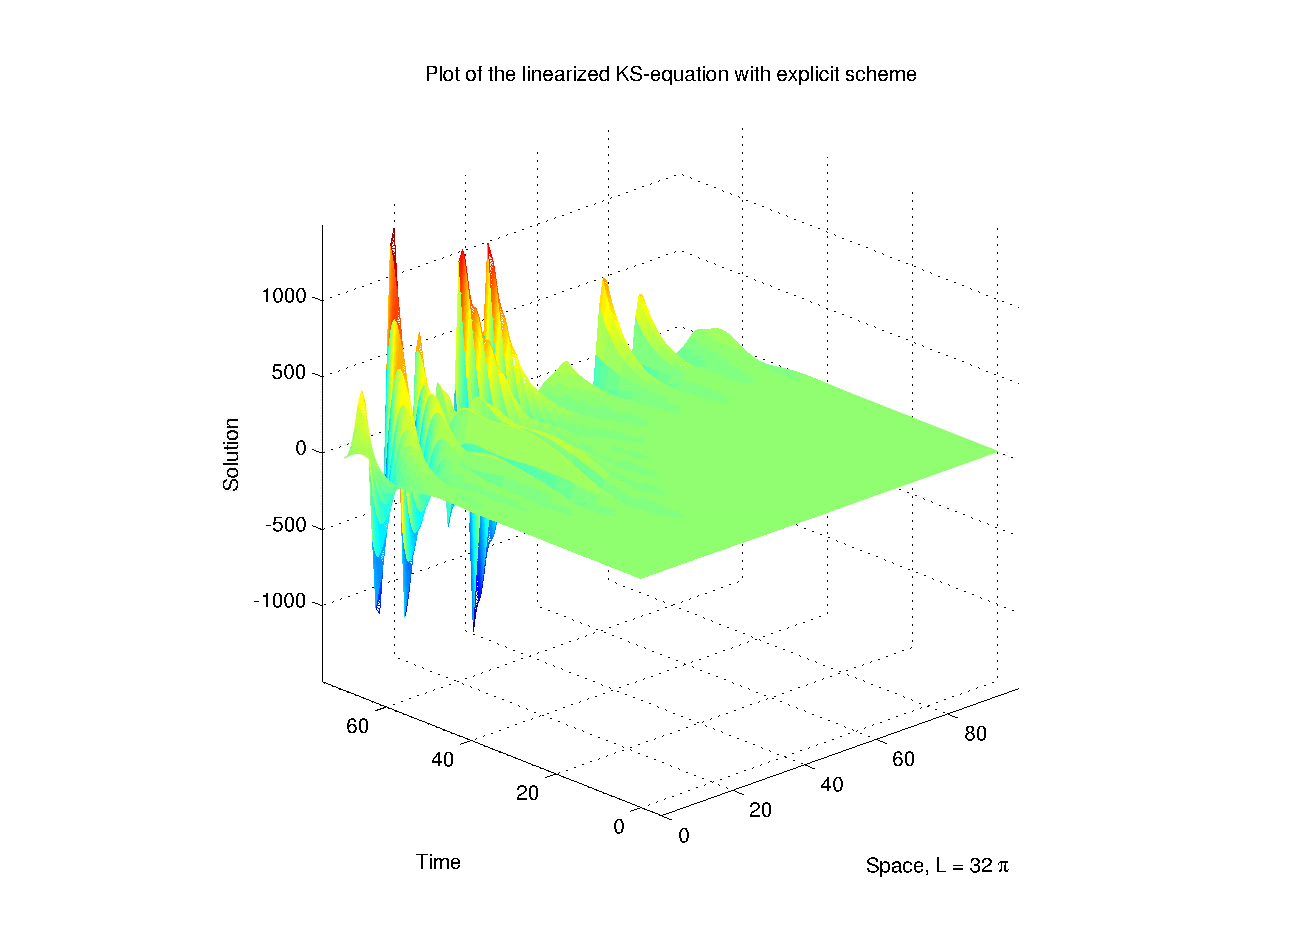
\includegraphics[scale=0.5]
{../PDFs/FE_Exp/linear_explicit.pdf}
\caption{Surface plot of $u(x,t)$ on the linearized explicit scheme. The method is unstable for all $r$.}
\label{fig:lin_exp}
\end{figure}









\section{Numerical results}
\subsection*{Initial conditions}
In the solution of the KS-equation we had periodic boundary conditions, i.e. $u(0,t) = u(L,t)$. We also used L-periodic initial conditions. We experienced that a common initial condition used in several other reports was

\begin{equation}
\label{initialCondition}
u(x,0) = \cos(\frac{x}{16})(1 + \sin(\frac{x}{16}).
\end{equation}

We also tried the initial condition

\begin{equation}
\label{initialCondition2}
u(x,0) = \frac{1}{\sqrt{2}} \sin(x) - \frac{1}{8}\sin(2x),
\end{equation}

which worked well. The L-periodic initial conditions is customarily taken \cite{periodicInitial} to satisfy

\begin{equation}
\int_0^L\! f(x)\,\textrm{d}x = 0,
\end{equation}
which both of our initial conditions satisfy. The same article also states that for L-periodic initial data, a unique solution for \eqref{KSeq} exits, and is bounded as $t\rightarrow\infty$. The bound has been proven to be smaller than $O(L^{8/5})$. In our numerical tests, with $t=5000$, the initial condition \eqref{initialCondition} did indeed not exceed the bound, nor did \eqref{initialCondition2}.

\subsection*{Plots of the function}
The IMEX method produced figure \ref{fig:surface}.

\begin{figure}[H]
\centering
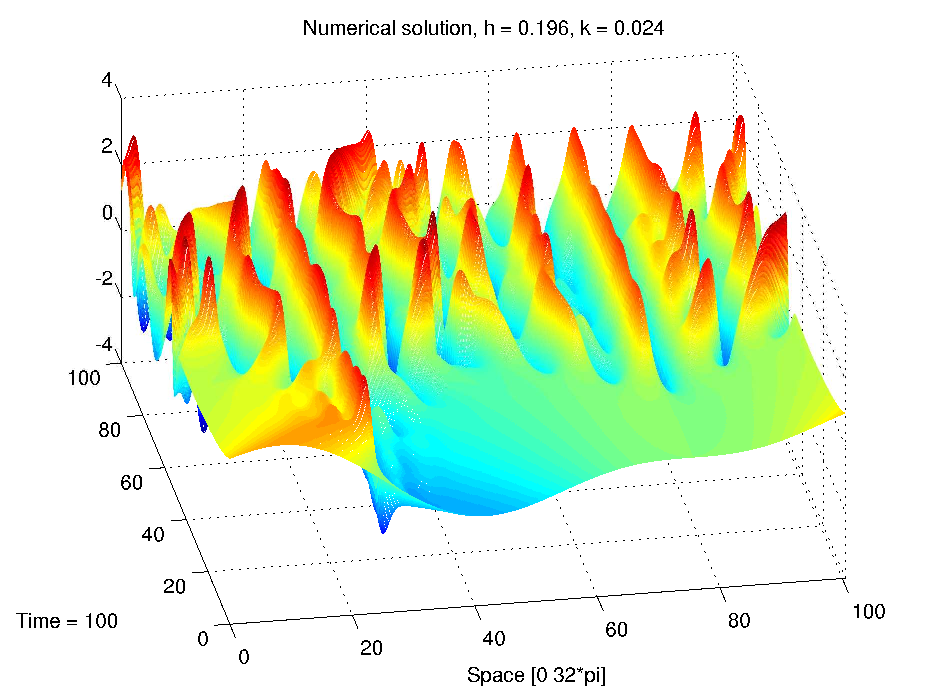
\includegraphics[scale=0.7]
{../PDFs/IMEX/KS_plot_surface.pdf}
\caption{Surface plot of the solution u(x,t)}
\label{fig:surface}
\end{figure}

As we can see, there are two parallel lines where the solution is symmetric in an interval around them. This is easier seen from the contour plot, figure \ref{fig:contour}.

\begin{figure}[H]
\centering
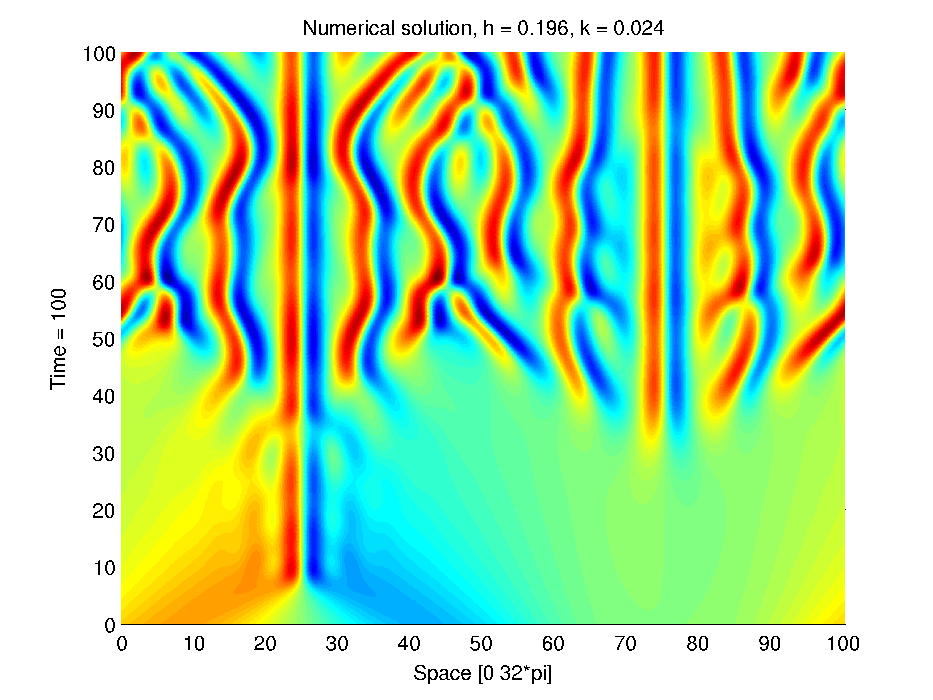
\includegraphics[scale=0.65]
{../PDFs/IMEX/KS_plot_contour.pdf}
\caption{Contour plot of the solution u(x,t)}
\label{fig:contour}
\end{figure}

Although the lines are parallel from time $t = [0,100]$, this ends after a time $t \thickapprox 250$, and it becomes even more chaotic.

Because \eqref{KSeq} has no analytical solution, we constructed a reference solution. Since our equation is stiff, we used the ODE15s solver to compute the solution, as this is particularly good for stiff systems. A semi-discretization, i.e. only discretization in space, was used in the solver. By using low values for $k$ and $h$, typically $k = 0.006$ and $h = 0.025$, we are confident that the solver produces a good approximation of the result. To see exactly how well our numerical solution is compared to the reference solution, we plotted the error between them. This produced figure \ref{fig:errPlots}.

\begin{figure}[H]
        \centering
        \begin{subfigure}[b]{0.52\textwidth}
                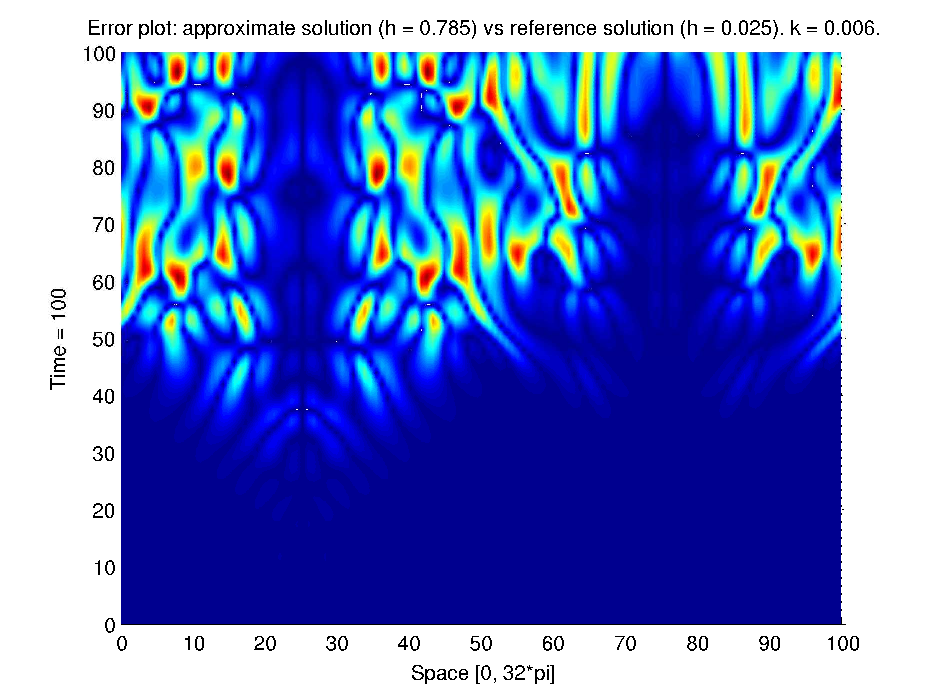
\includegraphics[width=\textwidth]{../PDFs/IMEX/error_num_ref_t100_3rd.pdf}
                \caption{Numerical solution, $h = 0.785$}
                \label{fig:highError}
        \end{subfigure}%
        ~ %add desired spacing between images, e. g. ~, \quad, \qquad etc.
          %(or a blank line to force the subfigure onto a new line)
        \begin{subfigure}[b]{0.52\textwidth}
                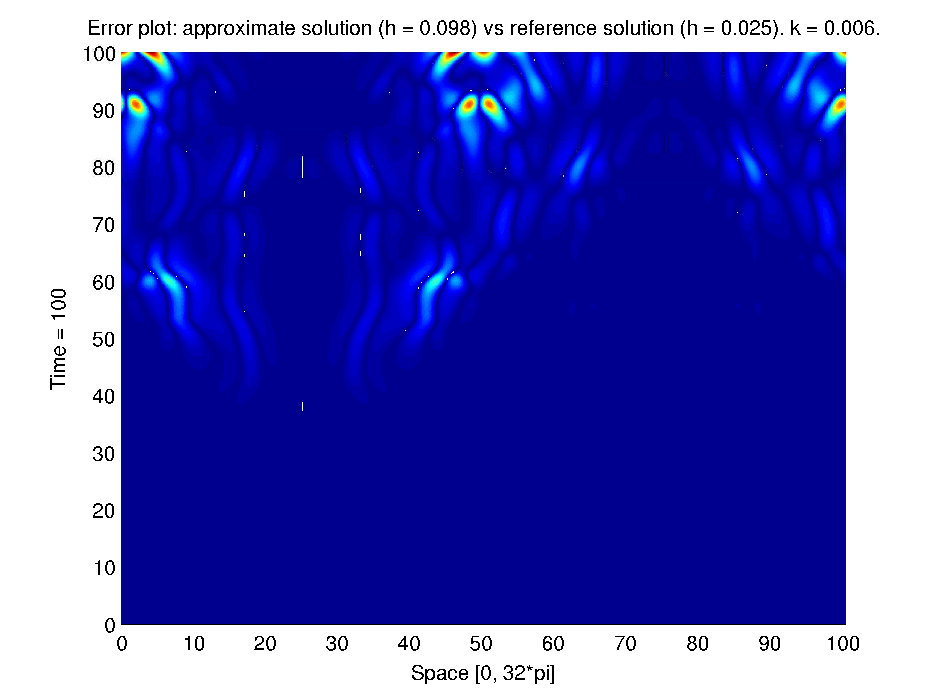
\includegraphics[width=\textwidth]{../PDFs/IMEX/error_num_ref_t100_1st.pdf}
                \caption{Numerical solution, $h = 0.098$}
                \label{fig:lowError}
        \end{subfigure}
        \caption{Comparison of the error between the reference solution and the numerical approximation for different $h$-values. Reference solution: $h = 0.025$, $k = 0.006$. Blue color shows low error, while red shows high error.}\label{fig:errPlots}
\end{figure}

As we can see, the error decreases when the $h$-value is decreased. A plot of the reference solution vs. our numerical solution, figure \ref{fig:errTime}, explains in a good way why some points have higher error than others. At the points where the reference solution and the numerical solution are out of phase, the error will naturally be large.This means a worst case error will be the sum of the amplitudes of the solutions, and this tends to happen. Worth noting is the low error at the two parallel lines, $x \thickapprox 25$ and $x \thickapprox 75$, which can also be seen in figure \ref{fig:errPlots}. 

\begin{figure}[H]
\centering
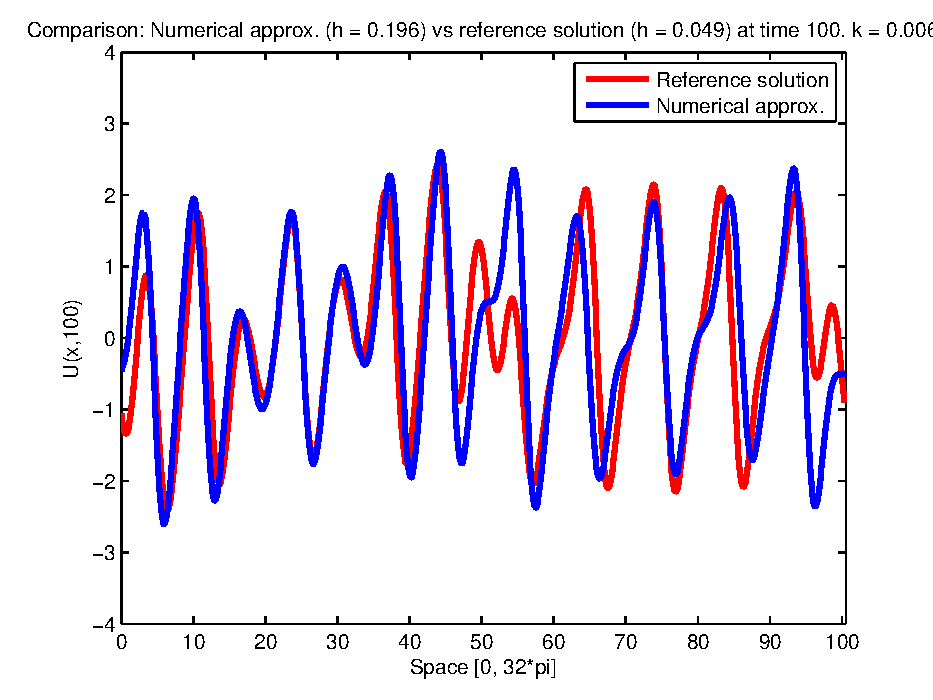
\includegraphics[scale=0.55]
{../PDFs/IMEX/comp_num_ref_t100.pdf}
\caption{Plot of $u(x,0)$ for the reference solution and the numerical solution}
\label{fig:errTime}
\end{figure}


\subsection*{Running time}

The implicit and explicit scheme both have negative and positive properties. While the explicit scheme is about 10 times faster than the implicit scheme, as shown in Figure \ref{fig:runTime}, it is has a restriction on the time step. In addition, it seems that the error is larger in the explicit scheme than the implicit scheme, independent on the number of time steps. 

\begin{figure}[H]
\centering
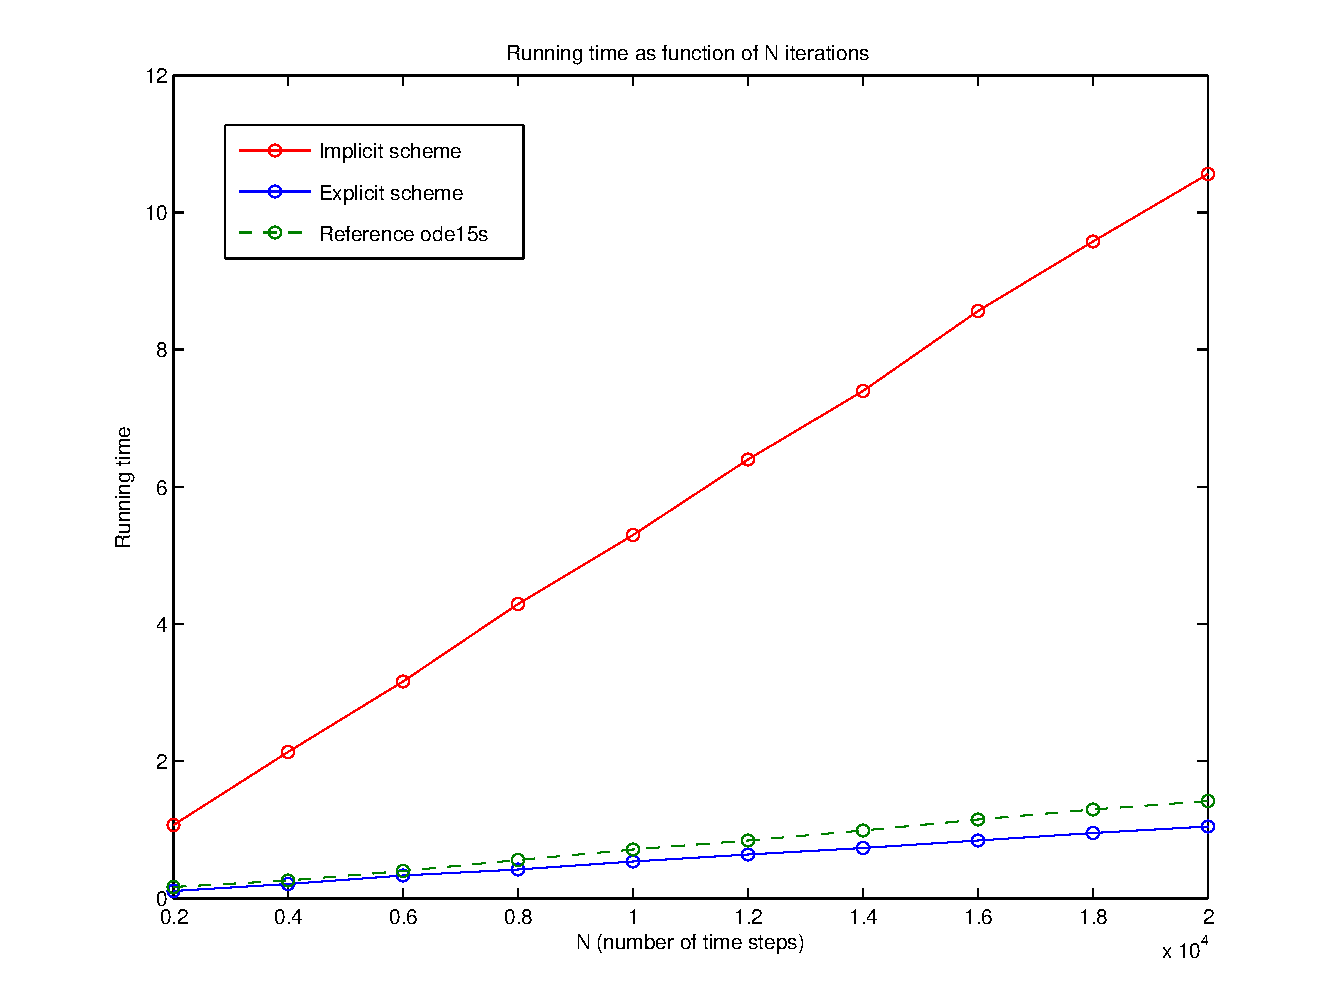
\includegraphics[scale=0.4]
{../PDFs/Comparisons/running_time3.pdf}
\caption{Running time of the two schemes as a function of time steps $N$}
\label{fig:runTime}
\end{figure}

\begin{figure}[H]
\centering
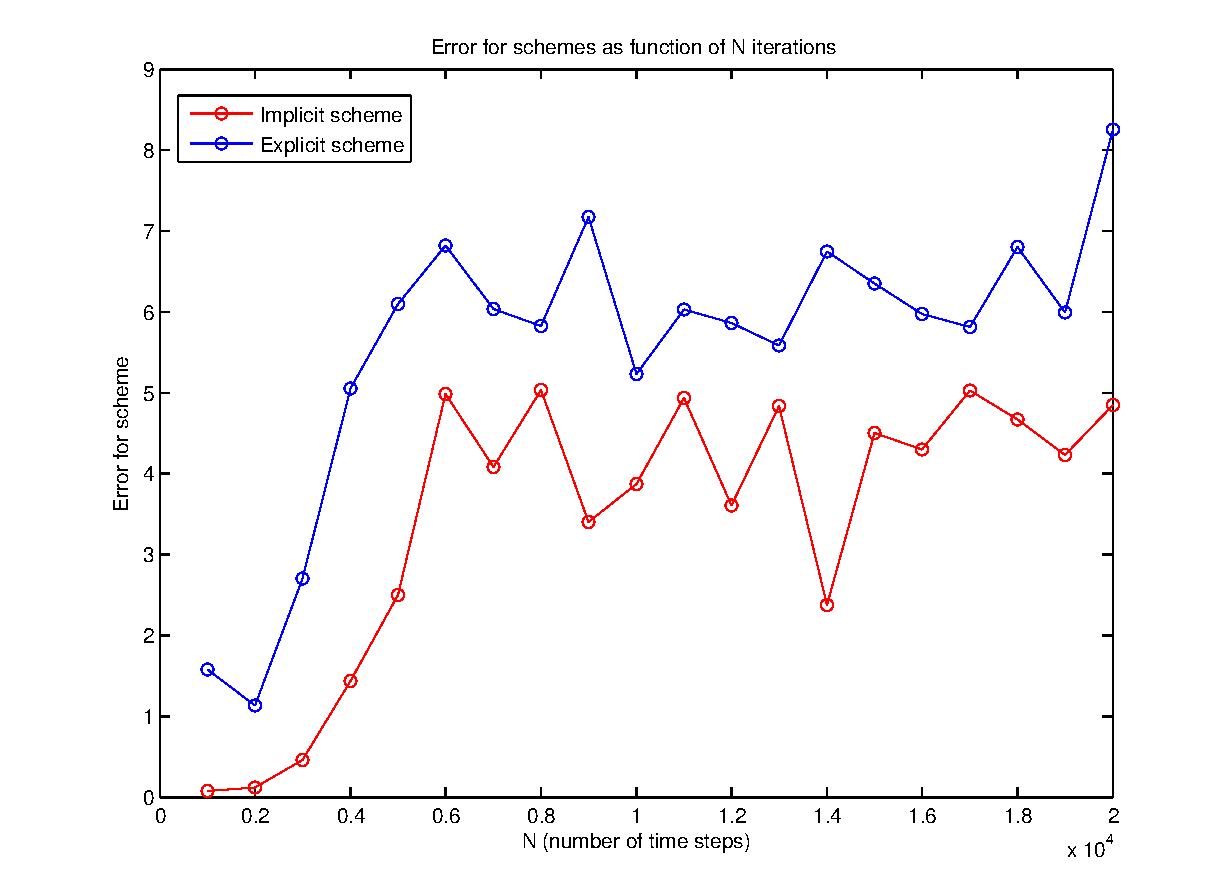
\includegraphics[scale=0.4]
{../PDFs/Comparisons/error_compare.pdf}
\caption{Running time of the two schemes as a function of time steps $N$}
\label{fig:runTime}
\end{figure}



\section{Conclusion}
By what we have seen from the numerical experiments, when comparing the two difference schemes, the implicit scheme shows better properties regarding stability than the explicit scheme. For the latter a stability criterion for the time step, $k/h^4 \le 1/8$, was given under some assumptions, but this time step is very low and unpractical. For the implicit method, we were not able to give any analytic reasonable criterion, but numerical testing implied stability for time steps smaller than $\frac{1}{3}$. Though the numerical computations are much more time consuming for the implicit method, due to the stiffness and instability of the system, this method would serve better in practice for modeling this equation.

When it comes to the collaboration in the group, it has been a real delight. We have known each other for a very long time and have worked together on several projects prior to this project. Even though we experienced trouble with the equation at times, we overcame the obstacles as a team, and both helped, and learned from each other. We split the workload in equal parts, and worked together the entire time. We feel that our interest in numerical mathematics has increased during the project, and we all feel that we have learned so much during the last couple of months.



\begin{thebibliography}{9}

\bibitem{development}
Scott Arthur Gasner, Fall 2004,
\emph{Integrating the Kuramoto-Sivashinsky equation: A simulation of the hopping state}
http://terminus.sdsu.edu/thesis\_repository/ScottGasner\_2004\_Fall\_MS\_Comp\_Sci.pdf, 03/31-2014

\bibitem{trivia}
Mehrdad Lakestani and Mehdi Dehghan, February 2012,
\emph{Numerical solutions of the generalized Kuramoto-Sivashinsky equation using B-spline functions},
http://www.sciencedirect.com/science/article/pii/S0307904X11004082, 03/31-2014

\bibitem{stabil}
Marjan Uddin and Sardar Ali, January 2013,
\emph{RBF-PS method and Fourier Pseudospectral method for solving stiff 
nonlinear partial differential equations},
http://www.naturalspublishing.com/files/published/ed38fj6n3xt187.pdf, 03/31-2014

\bibitem{periodicInitial}
Andrew Spratley, March 2010,
\emph{Kuramoto-Sivashinsky equation: A PDE with chaotic solutions},
http://people.maths.ox.ac.uk/trefethen/pdectb/kuramoto2.pdf, 03/31-2014

\bibitem{sparse}
Matlab documentation: computational advantages,
\emph{Computational Advantages},
http://www.mathworks.se/help/matlab/math/computational-advantages.html, 04/02-2014

\bibitem{ode15s}
Matlab documentation: ode15s,
\emph{ode15s},
http://www.mathworks.se/help/matlab/ref/ode15s.html, 04/02-2014


\end{thebibliography}

%http://www.dtic.mil/dtic/tr/fulltext/u2/a228590.pdf
\end{document}